\section{Experimental Evaluation}

To evaluate the performance of Viscous, we compare the Viscous with popular transport protocols MPTCP, MPQUIC, TCP and QUIC with different network configurations. We use the Mininet platform to perform most of our experiments. The mininet provides capability of generating different type of network topology with different network conditions in a single system and run any existing real network application on the Mininet generated network. We also performs few experiments on physical network using Raspberry Pi board.

For the Mininet based experiments, we use a computer with 8GB RAM, 4 core GenuineIntel i5-4590 CPU with 3.30 GHz clock frequency. It is equipped with Ubuntu 16.04.1 operating system with Linux kernel version 4.4.70 with the MPTCP v0.92 and the Mininet 2.2.2. For the Rapsberry pi setup, we use Raspberry Pi model 3.
To compare with the QUIC and the MPQUIC, we use golang implementation of the MPQUIC by Conick {\it et. al.}\cite{mpquic-measure} which is a extension of golang implementation of the QUIC\cite{quic-go}.

In rest of this section, we will produced different experiments and analysis of their results.

\begin{figure}
	\centering
	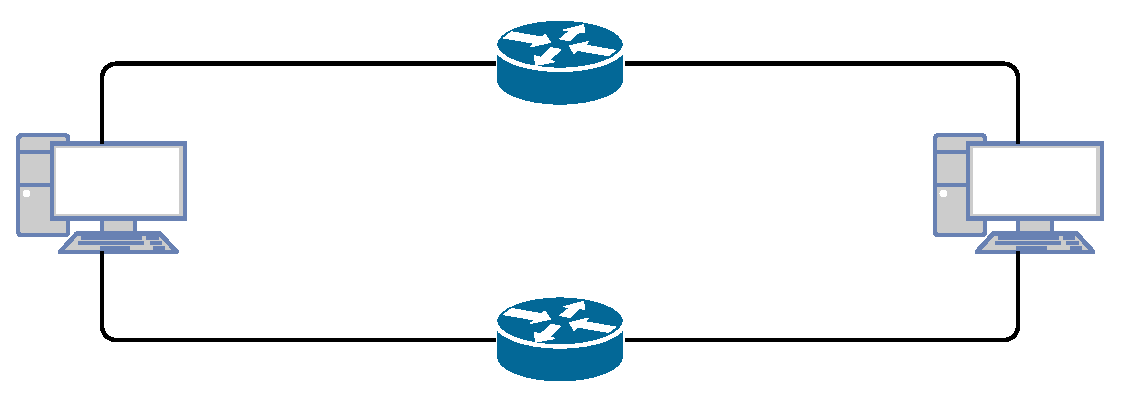
\includegraphics[width=\linewidth]{img/aggregation.eps}
	\caption{\label{fig:aggregation_dia}Network used to find aggregative benefit}
\end{figure}

\begin{table}[h]
	\centering
	\begin{tabular}{l||c|c||c|c}
		%		\hline
		& \multicolumn{2}{c||}{Low-BDP} & \multicolumn{2}{c}{High-BDP}\\
		\hline
		\hline
		Capacity [Mbps] & 0.1 & 100 & 0.1 & 100 \\
		\hline
		Propagation delay [ms] & 0 & 50 & 0 & 400 \\
		\hline
		Queuing [ms] & 0 & 100 & 0 & 2000 \\
		\hline
		Loss rate [\%] & 0 & 2.5 & 0 & 2.5 \\
		%		\hline
	\end{tabular}
	\caption{\label{tbl:noloss_param}Scenario used}
\end{table}

\begin{equation} \label{eqn:agre_benefit}
Bes(S) = 
\begin{cases}
\frac{G_v - G_p^{max}}{G_v - G_v^{max}} & \text{if} G_v > G_V^{max} \\
\frac{G_v - G_p^{max}}{G_v^{max}} & \text{otherwise}
\end{cases}
\end{equation}

\subsection{Measuring aggregated benefit}
To compare Viscous with other protocol in various network conditions, we perform similar experiment performed by \cite{mpquic-measure,Paasch:mptcp:compare}. We perform these experiments with various number of scenario by changing basic network parameters {\it e.g.} link bandwidth, RTT, queuing delay and packet loss rate. These experiments are performed using simple topology shown in Fig.~\ref{fig:aggregation_dia} with the help of Mininet network emulator. We run experiments on 143 scenario generated using WSP	space filling algorithm described in \cite{wspalgo} from configuration space described in Table~\ref{tbl:noloss_param}. Three experiment performed on each scenario for each protocols. We run experiments on TCP and QUIC for both the paths and compared with best performance. We also observed that the MPTCP depends on initial path selection, so we run experiments with MPTCP for both the path and compared with best and worst initial path performance. We considered GoodPut as the metric of performance. In each of these experiments, we send 50 back-to-back request-response over a single thread. The client request for a data-size to server and the server transfer the requested amount of data to client. We vary response size with a exponential distribution with mean 25KB\footnote{We decided 25KB as our initial observation with rich website yeld mean response size near 25KB.} payload.

To measure aggregative benefit, we followed modified equation provided in \cite{Kaspar:2012:MAH:2206765.2206770,Paasch:mptcp:compare,mpquic-measure}
as Equation~\ref{eqn:agre_benefit}. Here we measure the benefit of using Viscous instead of other protocol for a given scenario $S$. Here $G_v$ is the mean GoodPut found in all experiments using Viscous for the scenario $S$, $G_p^{max}$ is the max of mean GoodPut found in each path for single path protocol while $G_p^{max}$ is mean GoodPut achieved by a multipath protocol. The value of $Ben(S)$ is in between -1 to 1, while -1 mean GoodPut of other protocol is twice good as Viscous while 1 mean, GoodPut of other protocol is 0, and if $Ben(S)$ is 0, other protocol perform exactly same as Viscous. In Fig.~\ref{fig:benefit} and Fig.~\ref{fig:benefit-high}, we depicted the results of this experiment.

\begin{figure}
	\captionsetup[subfigure]{}
	\begin{center}
		\subfloat[\label{fig:benefit-box} Benefit of Viscous over other transport different protocol]{
			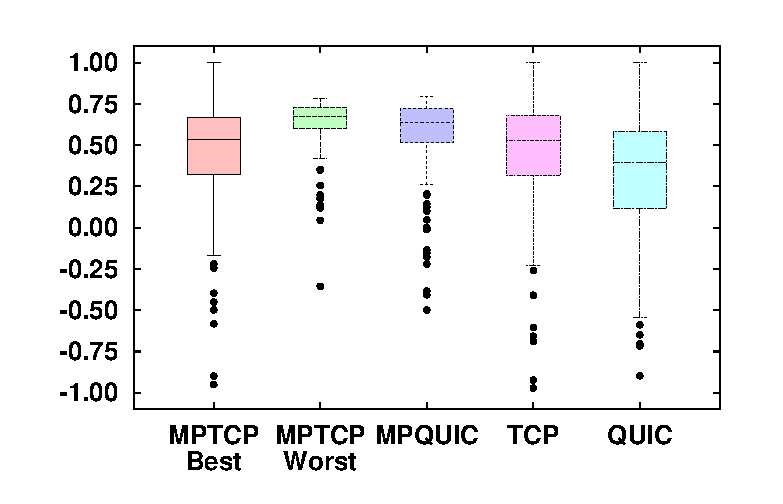
\includegraphics[width=.49\linewidth]{img/lowbdp-lossless/lowbdpnoloss_benefit.eps}
		}
		\subfloat[\label{fig:benefit-cdf} CDF of benefit of Viscous over other transport different protocol]{
			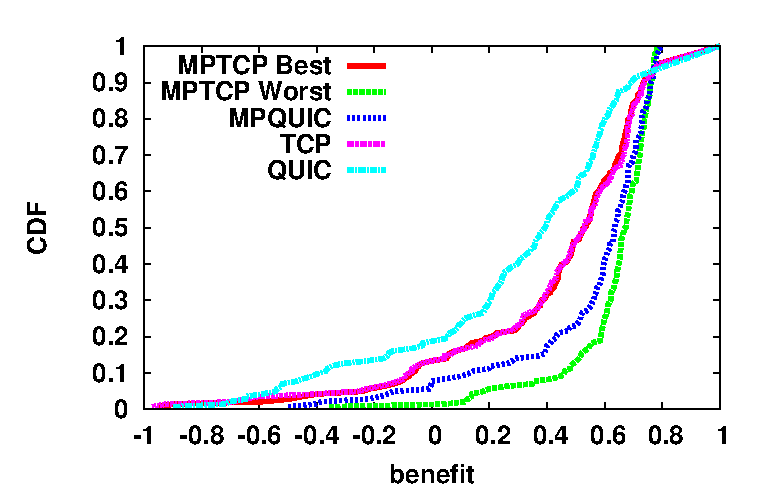
\includegraphics[width=.49\linewidth]{img/lowbdp-lossless/lowbdpnoloss_cdf.eps}
		}
		\caption{\label{fig:benefit}Experimental results on lossless low BDP channels}
	\end{center}
\end{figure}

We can see that the Viscous is performing better than all the other protocols. It can be understood that, the TCP and the MPTCP aren't performing good enough because they need to go through slow-start phase for every request. However it was not easy to find out the performance degradation of the QUIC or the MPQUIC. After taking close look to we found that congestion window have a limiting factor of 3.5MB in case of QUIC and MPTCP. This limiting factor is reducing the speed for the QUIC and MPQUIC while the Bandwidth or the RTT of the link is little higher. However, we kept no such limiting factor as speed is much more precious, the Viscous can have $cwnd$ size as high as the BDP for a channel.

\begin{figure}
	\captionsetup[subfigure]{}
	\begin{center}
		\subfloat[\label{fig:benefit-box-high} Benefit of Viscous over other transport different protocol]{
			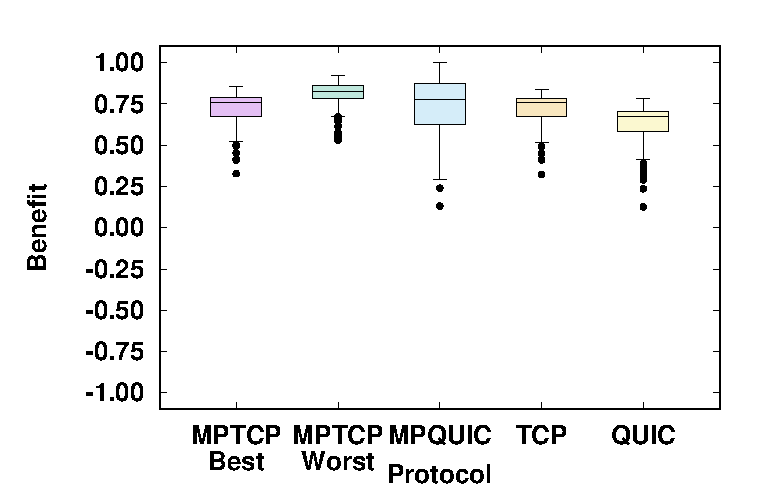
\includegraphics[width=.49\linewidth]{img/highbdp-lossless/highbdpnoloss_benefit.eps}
		}
		\subfloat[\label{fig:benefit-cdf-high} CDF of benefit of Viscous over other transport different protocol]{
			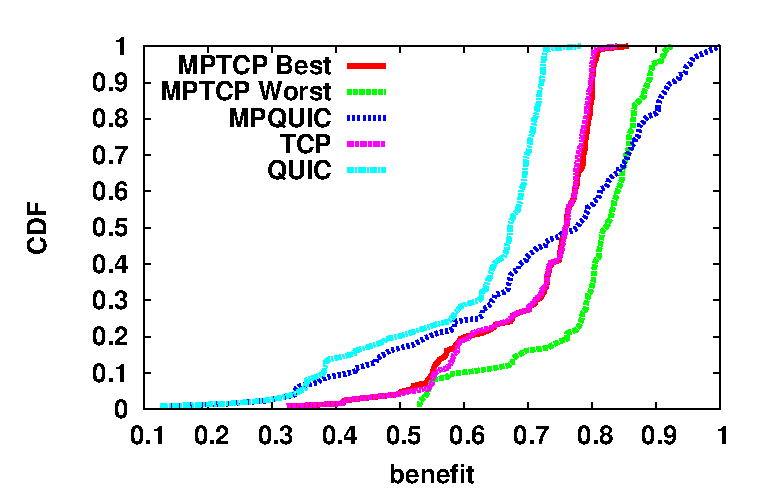
\includegraphics[width=.49\linewidth]{img/highbdp-lossless/highbdpnoloss_cdf.eps}
		}
		\caption{\label{fig:benefit-high}Experimental results on lossless high BDP channels}
	\end{center}
\end{figure}


%======================================
% place holder for experiments on lossy channels
%======================================
\begin{figure}
	\captionsetup[subfigure]{}
	\begin{center}
		\subfloat[\label{fig:benefit-box-lossy} Benefit of Viscous over other transport different protocol]{
			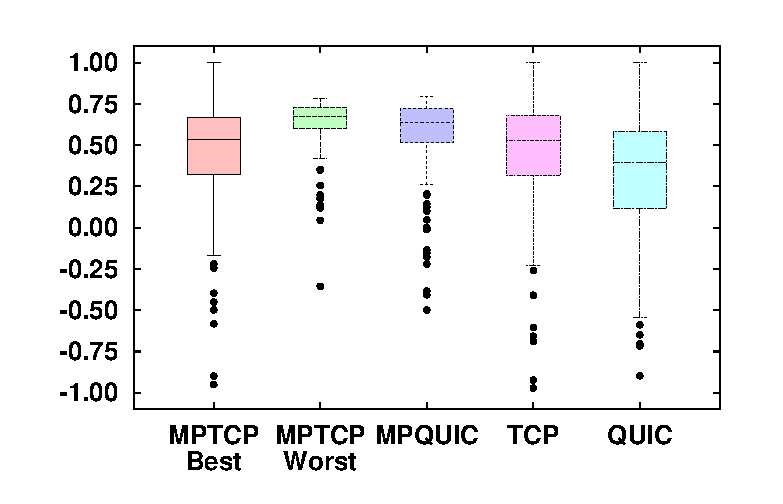
\includegraphics[width=.49\linewidth]{img/lowbdp-lossless/lowbdpnoloss_benefit.eps}
		}
		\subfloat[\label{fig:benefit-cdf-lossy} CDF of benefit of Viscous over other transport different protocol]{
			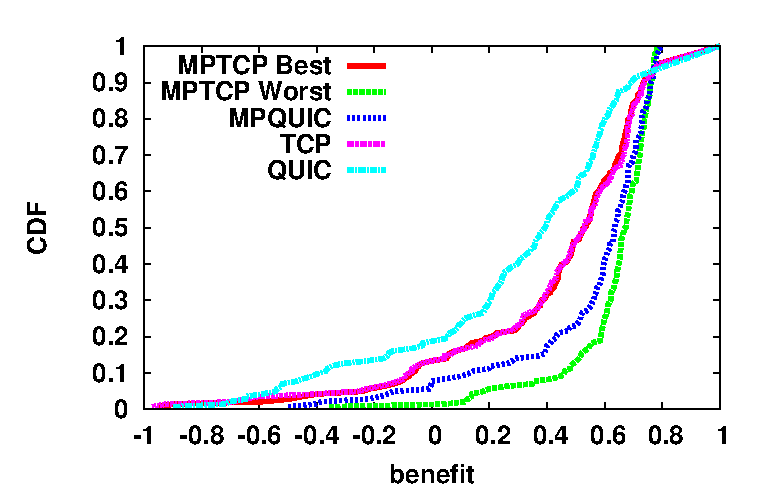
\includegraphics[width=.49\linewidth]{img/lowbdp-lossless/lowbdpnoloss_cdf.eps}
		}
		\caption{\label{fig:benefit-lossy}(\noteam{placeholder})Experimental results on lossy low BDP channels}
	\end{center}
\end{figure}

\begin{figure}
	\captionsetup[subfigure]{}
	\begin{center}
		\subfloat[\label{fig:benefit-box-high-lossy} Benefit of Viscous over other transport different protocol]{
			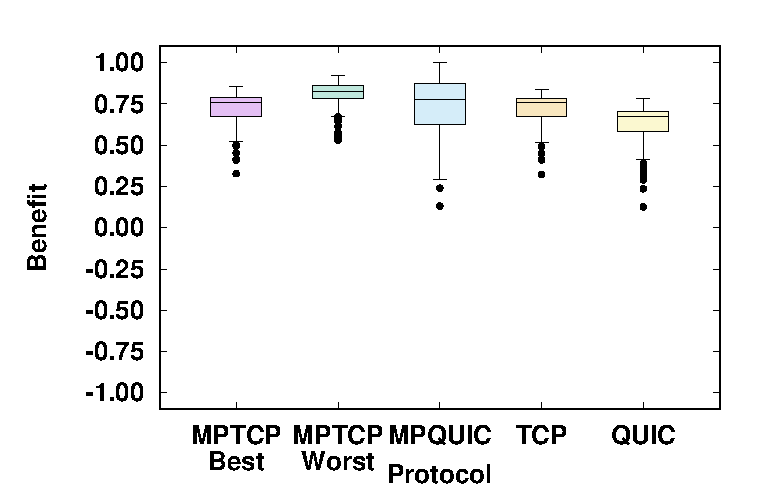
\includegraphics[width=.49\linewidth]{img/highbdp-lossless/highbdpnoloss_benefit.eps}
		}
		\subfloat[\label{fig:benefit-cdf-high-lossy} CDF of benefit of Viscous over other transport different protocol]{
			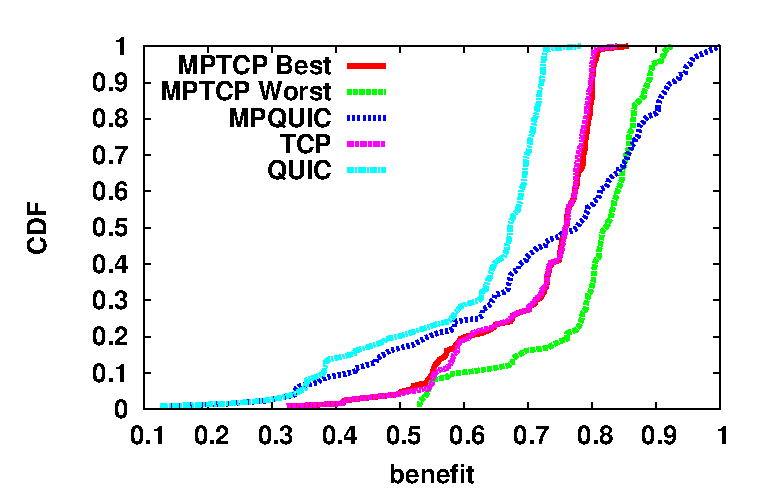
\includegraphics[width=.49\linewidth]{img/highbdp-lossless/highbdpnoloss_cdf.eps}
		}
		\caption{\label{fig:benefit-high-lossy}(\noteam{placeholder})Experimental results on lossy high BDP channels}
	\end{center}
\end{figure}

%======================================
% place holder for experiments on lossy channels
%======================================

\begin{figure*}[h]
	\captionsetup[subfigure]{}
	\begin{center}
		\subfloat[\label{fig:rocketfuel_time_5_20}Delay=5ms \#threads=5]{
			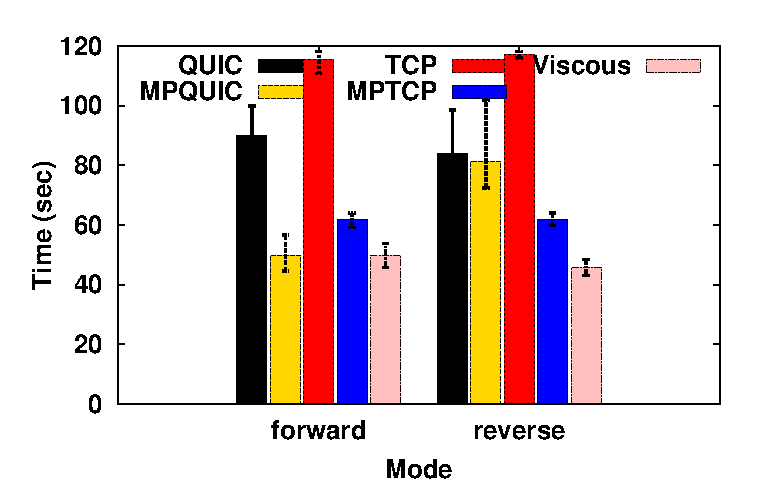
\includegraphics[width=0.24\linewidth]{img/rocketfuel/tymdiff-5-5.eps}
		}
		\subfloat[\label{fig:rocketfuel_time_10_5}Delay=10ms \#threads=5]{
			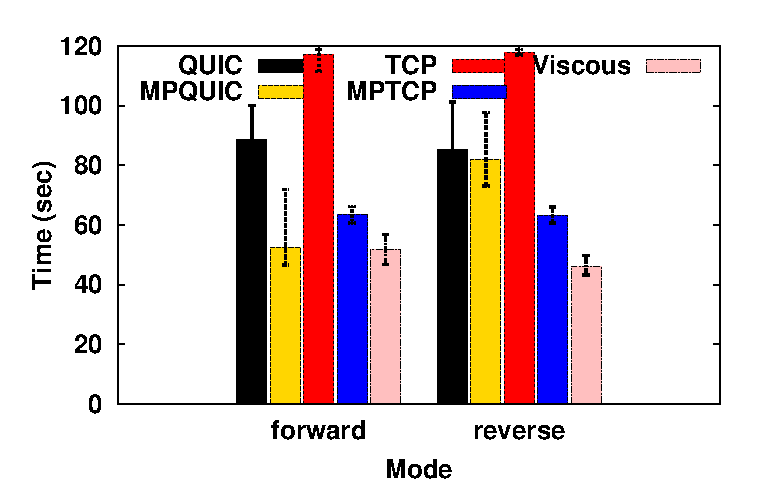
\includegraphics[width=0.24\linewidth]{img/rocketfuel/tymdiff-10-5.eps}
		}
		\subfloat[\label{fig:rocketfuel_time_10_20}Delay=10ms \#threads=20]{
			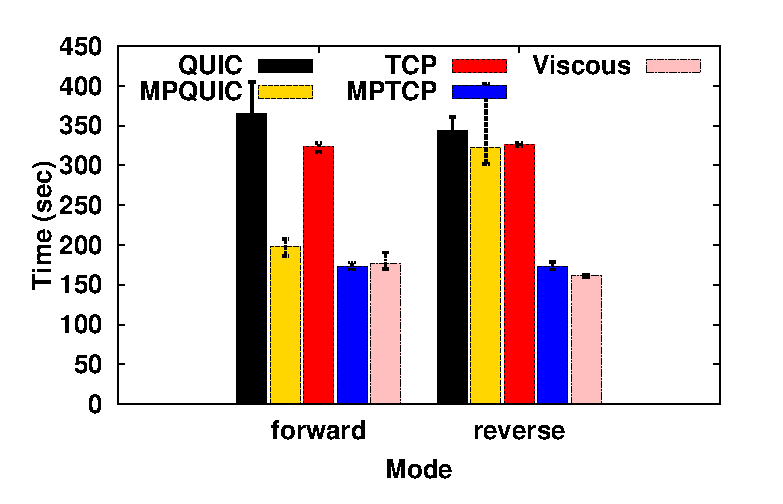
\includegraphics[width=0.24\linewidth]{img/rocketfuel/tymdiff-10-20.eps}
		}
		\subfloat[\label{fig:rocketfuel_time_20_20}Delay=20ms \#threads=20]{
			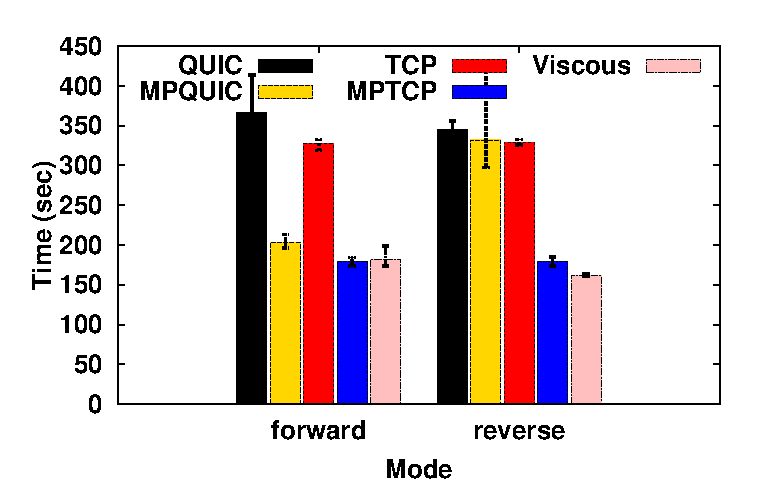
\includegraphics[width=0.24\linewidth]{img/rocketfuel/tymdiff-20-20.eps}
		}
		\caption{\label{fig:rocketfuel_time}Average average flow completion time over Rocketfuel topology}
	\end{center}
\end{figure*}


\begin{figure*}[h]
	\captionsetup[subfigure]{}
	\begin{center}
		\subfloat[\label{fig:rocketfuel_goodput_5_20}Delay=5ms \#threads=5]{
			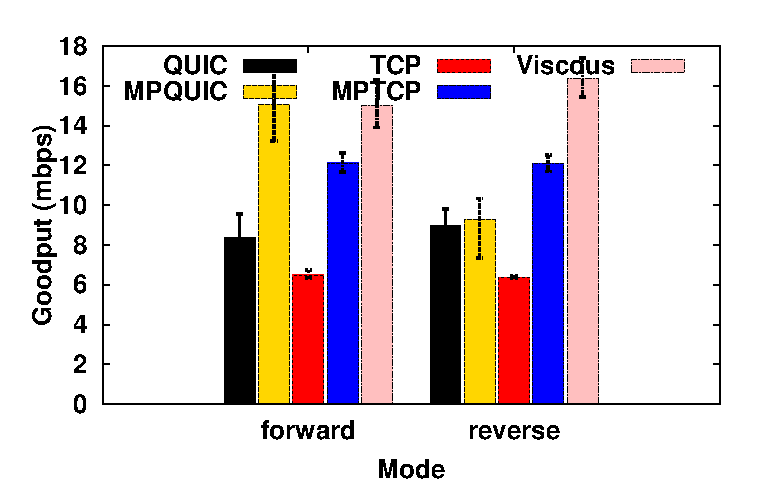
\includegraphics[width=0.24\linewidth]{img/rocketfuel/goodPut-5-5.eps}
		}
		\subfloat[\label{fig:rocketfuel_goodput_10_5}Delay=10ms \#threads=5]{
			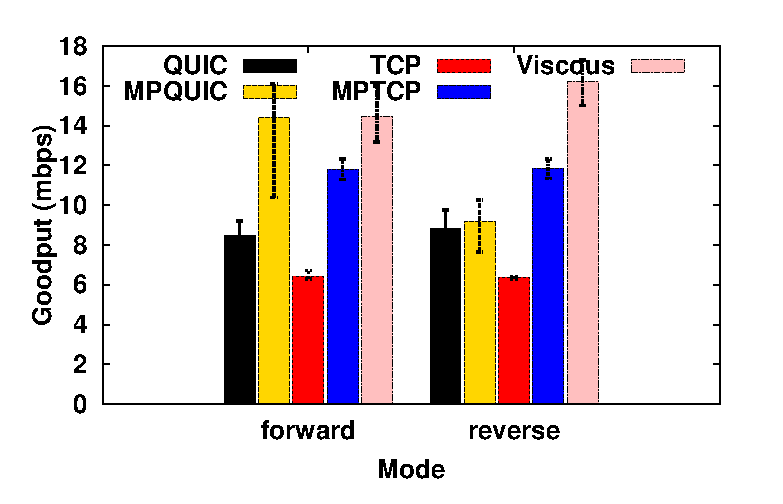
\includegraphics[width=0.24\linewidth]{img/rocketfuel/goodPut-10-5.eps}
		}
		\subfloat[\label{fig:rocketfuel_goodput_10_20}Delay=10ms \#threads=20]{
			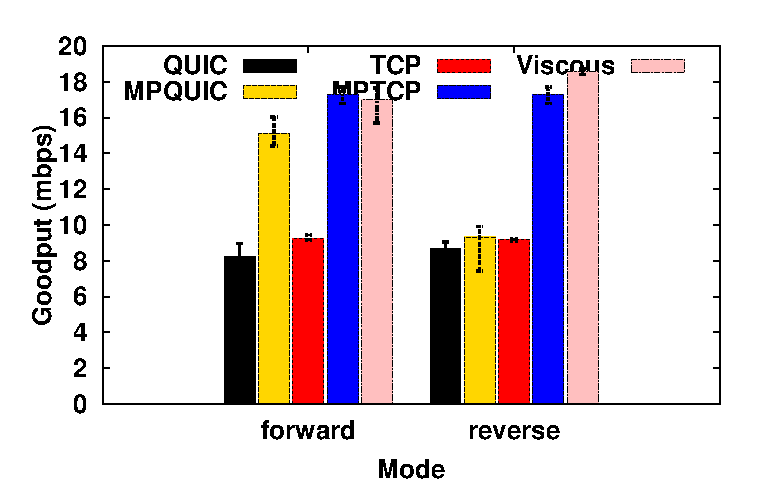
\includegraphics[width=0.24\linewidth]{img/rocketfuel/goodPut-10-20.eps}
		}
		\subfloat[\label{fig:rocketfuel_goodput_20_20}Delay=20ms \#threads=20]{
			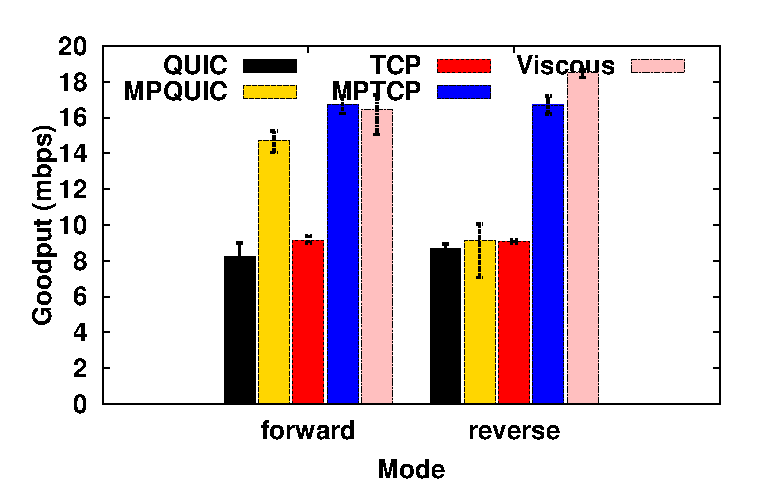
\includegraphics[width=0.24\linewidth]{img/rocketfuel/goodPut-20-20.eps}
		}
		\caption{\label{fig:rocketfuel_goodput}Average GoodPut over Rocketfuel topology}
	\end{center}
\end{figure*}

\subsection{Performance on overlapped path with RocketFuel topology}
The RocketFuel topology is a standard topology generated by using {\tt traceroute} from different locations all over the globe to different servers. We take a topology with 29 different networks connected via 15 routers. We place 14 host inside different networks. Among these 14 hosts, we connect 7 hosts with two different networks (we call it client host) and other 7 hosts with a single network (server host). So, there are 7 pair of server-client host. In this topology we use 3 different bandwidth for different links i.e. core link, server link, and client link. A core links connects a switch with a router with 100mbps bandwidth and 3ms delay, a server link connects a server and a switch with 50mbps bandwidth and 2ms delay. We keep 10mbps bandwidth for client link connecting a client host and a switch while varying the delay over different experiment.

In experiments, we sent data from each server host to their dedicated client host using different protocols (Viscous, QUIC, MPQUIC, TCP and MPTCP) and other way around. We call forward experiment when we send traffic from server host to client host and reverse experiment when we send data from client host to server host.

In this experiment, we vary client link delay and number of simultaneous thread. Then we send 50 back-to-connection through each thread with payload varied using exponential distribution with mean payload size 250kB. 


\begin{figure}
	\centering
	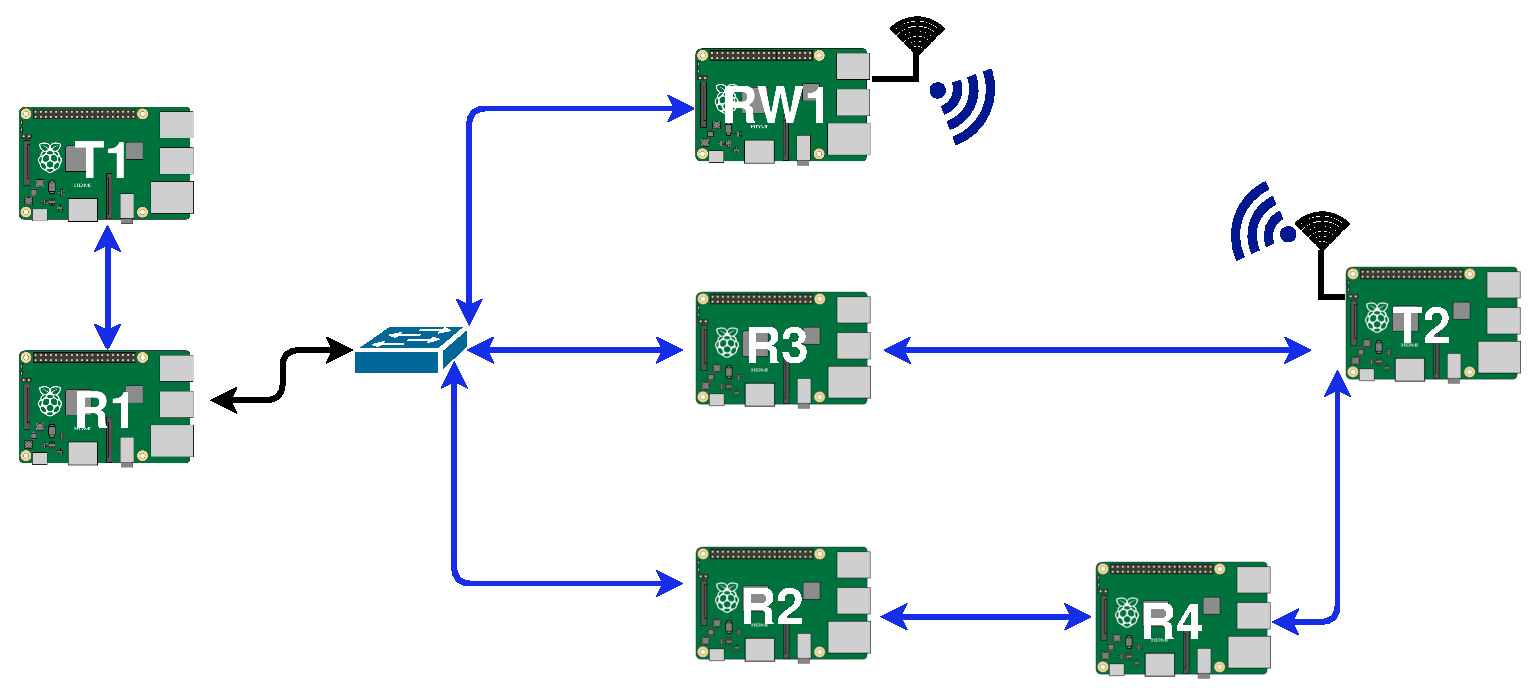
\includegraphics[width=.9\linewidth]{img/mobility/demo-Diagram.eps}
	\caption{\label{fig:mobility_diagram}Raspberry pi setup to test the mobility of viscous}
\end{figure}


\begin{figure*}[h]
	\centering
	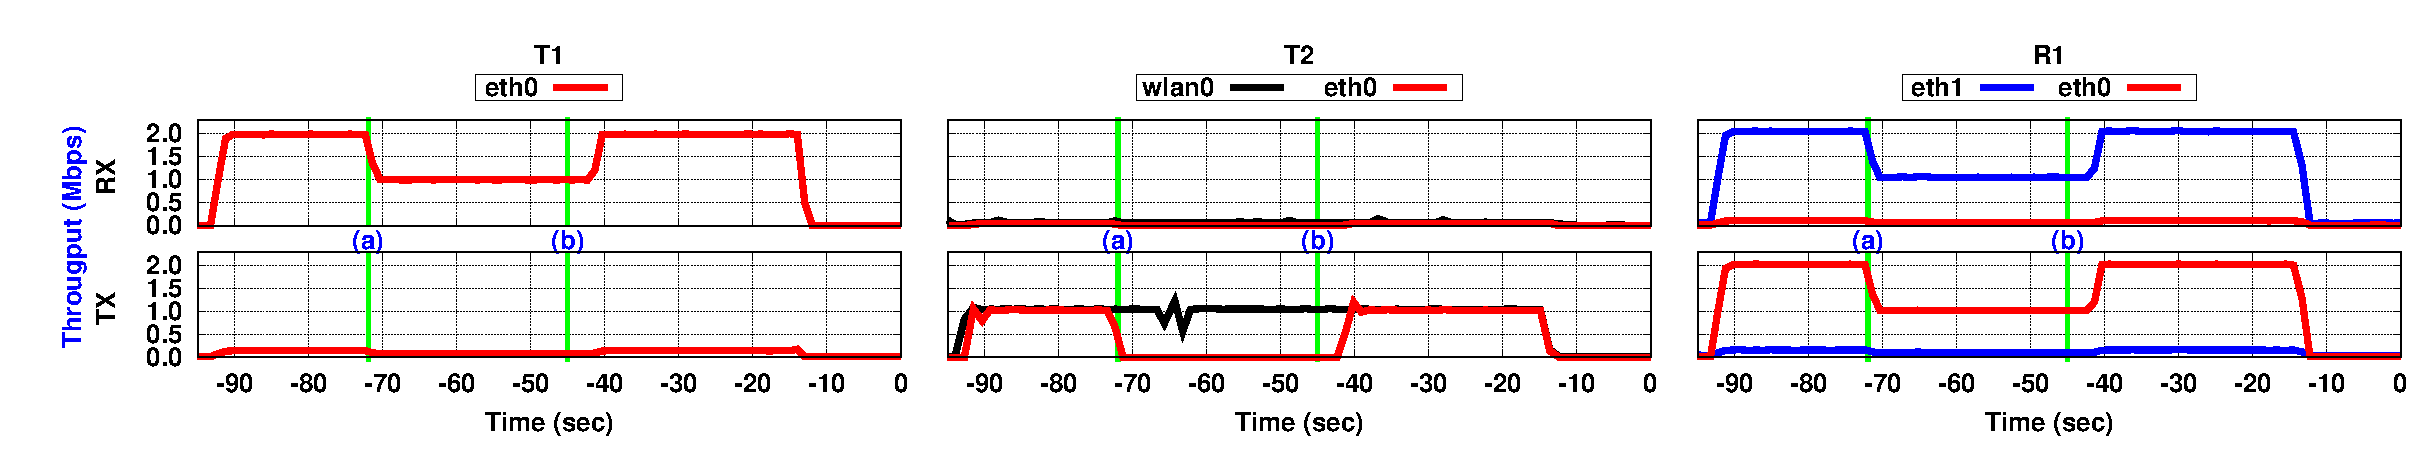
\includegraphics[width=\linewidth]{img/mobility/T1-T2-R1.eps}
	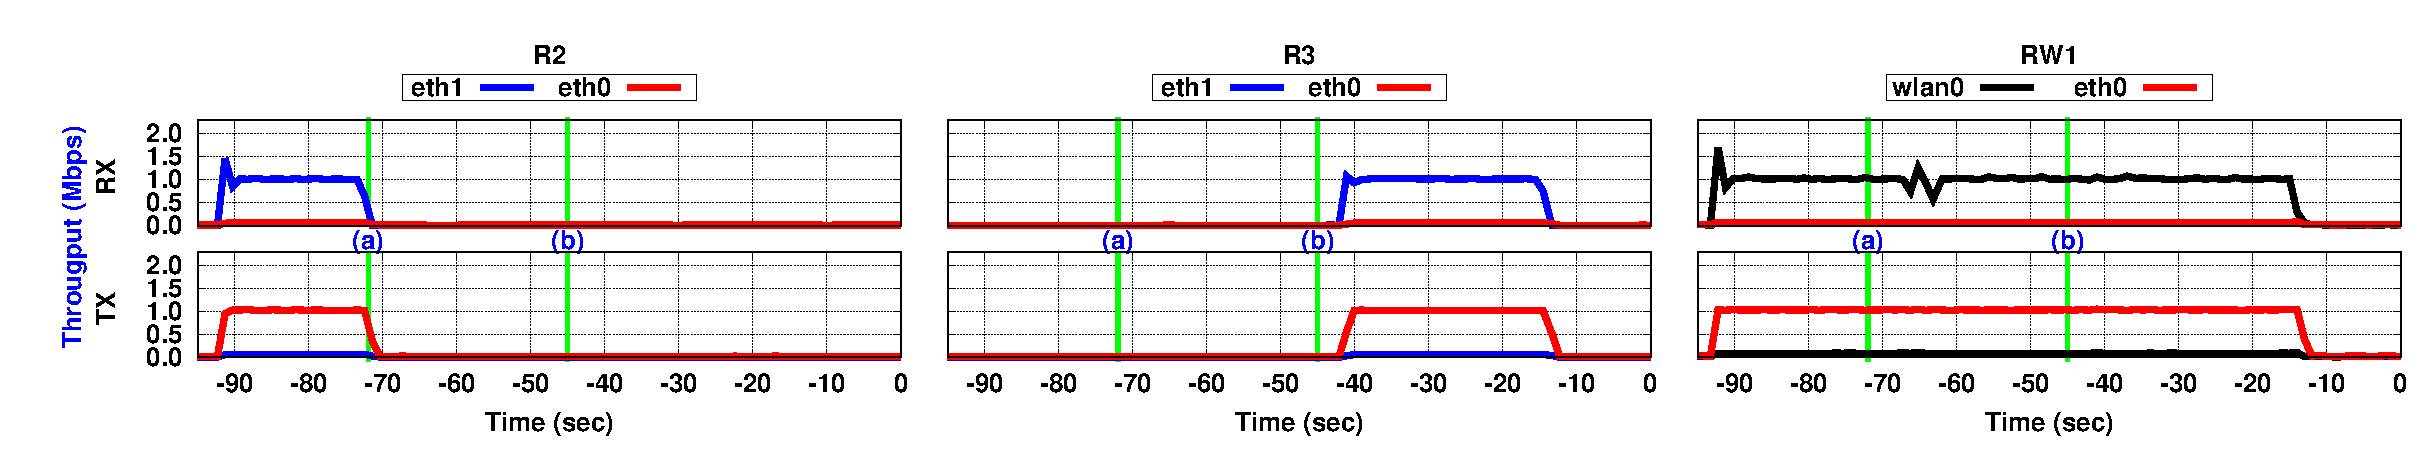
\includegraphics[width=\linewidth]{img/mobility/R2-R3-RW1.eps}
	\caption{\label{fig:mobility_res}RX-TX throughput at different hosts and routers}
\end{figure*}

In Fig.~\ref{fig:rocketfuel_goodput} and Fig.~\ref{fig:rocketfuel_time}, we have shown few selected results. There are two observation we can get from these plot. Firstly, In all of the cases, Viscous performs as good as the MPQUIC. In fact, the Viscous out performed the MPQUIC in reverse flow experiment. It is because Viscous is true multi-path-multi-stream protocol, while the QUIC is not a multi-path protocol. The MPTCP is not as multi-stream protocol, so it required new connection for each transmission. The MPQUIC is multi-path multi-stream protocol, but it suffers for reverse flow because, it can not take advantage of multiple interface during sending a datagram due the UDP api limitation. Viscous does not suffers in the reverse flow experiments because the Viscous use Packet-Socket api.


\subsection{Experiment on mobility}
We perform an experiment on mobility. To test this feature, we prepare the test platform using Raspberry Pi 3. We have depicted the setup diagram in Fig.~\ref{fig:mobility_diagram}. There are total five Raspberry pi acting as routers, this are R1, R2, R3, R4 and RW1. Two host T1 and T2 with this setup. The T1 host directly connected to R1. The host T2 connected to RW1 using WiFi channel. The T2 host is also connected to R3, R4 router via wire. The host T2 can stay connected with R4 or R3 at a time, not with both. All the links except link between RW1 and T2 in this setup are wired link.

To performs the experiment, we start sending data from T2 to T1 while T2 is connected with R4 via wired link and RW1 via WiFi. While the Viscous connection is live, we disconnect T2 from R4. After few seconds, we connect T2 with R3. 

We have shown the result in Fig.~\ref{fig:mobility_res}. In these plots, we have depicted in-coming (RX) and out-going (TX) throughput for each network interfaces for two hosts and 4 routers two covers all the paths between T1 and T2. Top plots depict RX throughput over time and bottom plot depict TX throughput over time for each hosts and routers. Now, we disconnect the link between R4 and T2 at -65th seconds (marked as {\tt a} in plots) and we connect T2 with R3 at time -55 seconds (marked as {\tt b} in plots).

We can see that the Viscous handles mobility pretty. It easily detect the closed link and turn off data transmission through that link. It can also detect new link and establish a channel through new link. We can see it takes few seconds to establish a new connection. It is happening because we are using external tool NetworkManager to provided network connection-disconnection event to the Viscous for now.
